\documentclass[journal=jprobs,manuscript=article,hyperref,doi=true]{achemso}
% ACS Journal of Proteome Research (JPR) submission template, built on the
% ACS-sanctioned achemso LaTeX class (CTAN, config achemso-jprobs.cfg,
% "J. Proteome Res.", v3.13g). achemso supplies the JPR layout, ACS numbered
% superscript citation style (natbib + achemso.bst), unnumbered section headings
% (\SectionNumbersOff for jprobs), keyword support, and the graphical
% Table-of-Contents (TOC) entry mechanism required for JPR articles.
\usepackage[utf8]{inputenc}
\usepackage[T1]{fontenc}
\usepackage{amsmath}
\usepackage{newtxtext,newtxmath}   % Times New Roman (metric-compatible) text + math
\usepackage{textcomp}
\usepackage{array}
\usepackage{microtype}
\usepackage{caption}
\hypersetup{colorlinks=true,allcolors=blue}
\frenchspacing
\widowpenalty=10000
\clubpenalty=10000
\displaywidowpenalty=10000
% Keep the reader-facing figure/table number in the caption.  The prior
% submission suppressed the label globally, which made a floated page hard to
% audit when several figures shared a page.  ACS's period separator gives the
% explicit ``Figure N.'' / ``Table N.'' form used by the text references.
\captionsetup{labelformat=default,labelsep=period,justification=justified,font=small,skip=5pt}
\emergencystretch=4em   % absorb the occasional long unbreakable token in justified text
\usepackage{xurl}  % break long \path names at / and _
% xurl supplies breakpoints inside long identifiers and SHA-256 strings.

% Visual-Ralph layout only (2026-09-11): tighten title skips; absorb leftover
% TOC page onto the leftover-refs page. Do not change title wording or science.
\makeatletter
\let\tableinput\@@input
\setlength{\acs@space@pre@title}{0pt}
\setlength{\acs@space@post@title}{0.75em}
\setlength{\acs@space@post@author}{0.55em}
\setlength{\acs@space@post@address}{0.55em}
\setlength{\acs@space@post@email}{0.55em}
\renewcommand{\acs@tocentry@print}[1]{%
  \gdef\acs@tocentry@text{\normalsize#1}%
  \AtEndDocument{\acs@tocentry@print@aux}%
}
\makeatother
\pdfminorversion=7

% Keep the four-line title compact so the abstract remains one unit.
% Body and abstract keep the class's review spacing.
\renewcommand{\titlefont}{\bfseries\sffamily\setstretch{1.15}}

\renewcommand{\topfraction}{0.85}
\renewcommand{\bottomfraction}{0.70}
\renewcommand{\floatpagefraction}{0.75}
\renewcommand{\textfraction}{0.10}

\title{Random cross-validation understates cross-cohort calibration error in multi-cohort proteomics: an accession-aligned
evaluation-protocol contrast}

\author{Zeyu Fu}
\altaffiliation{ORCID 0009-0001-8329-0108}
\email{fuzeyu99@126.com}
\affiliation[Army Medical University]
  {State Key Laboratory of Trauma and Chemical Poisoning, Institute of Combined Injury,
   Chongqing Engineering Research Center for Nanomedicine, College of Preventive Medicine,
   Army Medical University, Chongqing, China}

\keywords{proteomics; mass spectrometry; machine learning; cross-study validation;
model calibration; data leakage; CPTAC; selective prediction}

\hypersetup{pdfauthor={Zeyu Fu},pdftitle={Random cross-validation understates cross-cohort calibration error in multi-cohort proteomics: an accession-aligned evaluation-protocol contrast}}

\begin{document}

\begin{tocentry}
\centering
% Purpose-built single-panel TOC (ACS ≤ 3.25 in wide); replaces multi-panel F1 reuse.
% The confound disclosure is rendered INSIDE the art (panel title "A protocol contrast, not a
% proteomic transfer law" and the cancer/study confound), because ACS strips the
% graphical abstract from the article body and it is read on its own; see make_b28_figures.R.
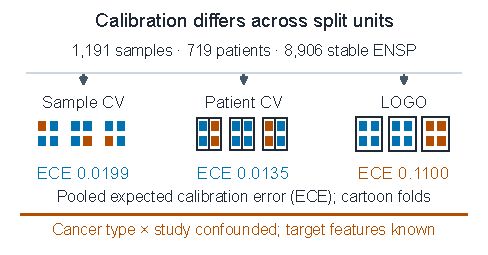
\includegraphics[width=3.25in]{figures/b28_TOC.pdf}
\end{tocentry}

\begin{abstract}
Cancer type and study are confounded in the six-cohort proteomics design examined here, so a protocol contrast cannot identify biological and acquisition effects separately. We audited tumor-versus-source-defined-normal classification in 1{,}191 CPTAC samples from 719 patients using 8{,}906 accession-aligned protein features. The shared feature intersection was defined using all six cohorts before evaluation, so LOGO is conditional on target-cohort feature availability rather than target-blind panel selection. Correcting cored-normal labels and patient identities, leave-one-cohort-out (LOGO) evaluation yielded equal-cohort macro AUROC 0.9343 and separately computed pooled AUROC 0.9555, with pooled ten-bin expected calibration error (ECE) 0.1100. Sample-stratified and true-patient-grouped five-fold cross-validation gave pooled AUROC 0.9942 and 0.9944, and ECE 0.0199 and 0.0135. Patient grouping did not erase the protocol gap. Missingness and three reference-normalized global summaries gave macro/pooled AUROC 0.5445/0.5116 and 0.8172/0.8492; differences from abundance are predictive increments, not biological signal fractions. Confidence-ranked abstention increased retained accuracy from 0.8497 to 119/119 at 10\% coverage, with 107 retained samples from two easier cohorts. Model and recalibration sensitivities showed cohort-dependent effects despite small pooled differences. The corrected evidence supports cohort-resolved evaluation of ranking, probability error and coverage in this design, not a deconfounded biological transfer estimate or clinical biomarker.
\end{abstract}

\section{Introduction}

This design cannot separate cancer-type biology from study-specific acquisition conditions. Each leave-one-cohort-out group is a distinct cancer/study cohort; the data do not establish that each cohort corresponds to one instrument, laboratory or acquisition run. Transfer discrimination and calibration therefore cannot be attributed to biology or technical effects alone \citep{LeekBatch}. The result is a protocol contrast under that confound, not a proteomic transfer law.

Quantitative mass-spectrometry proteomics now supports supervised classifiers for tumor status, subtype, and
related endpoints, and the Clinical Proteomic Tumor Analysis Consortium (CPTAC) has made harmonized proteomic data
for many cancer types openly available \citep{CPTACportal,CPTACpancancer}. When such a classifier is reported, its
performance is most often estimated by random $k$-fold cross-validation. In a multi-cohort proteomic dataset, that
protocol places samples from the same study cohort on both sides of the train/test split. Such a split answers an interpolation question; presenting it as an estimate of transfer to an unseen study can give an optimistic impression of generalization \citep{KapoorLeakage}. The practically relevant question is rarely ``how well does the model do on held-out
samples from the studies it was trained on'' but ``how well, and how reliably, does it transfer to a new
study'' --- which only a grouped, leave-one-study-out split estimates, and even then only as a protocol
contrast when cancer type and study are locked together. This inflation of within-study, random-split
performance relative to cross-study evaluation is not new to proteomics: cross-study validation frameworks
for genomic and transcriptomic prediction algorithms have previously shown that random cross-validation
within a pooled multi-study dataset systematically overestimates performance relative to leave-one-study-out
evaluation \citep{BernauCrossStudy}. Our contribution is to demonstrate this protocol difference on real
proteomics with a coupled discrimination-and-calibration analysis, not to report a new biological law.

Related work separates several causes of unreliable validation. The pipeML preprint recomputes
global features within folds and supports cohort-aware validation, including leave-one-dataset-out
analysis \citep{HurtadoPipeML}. Our audit addresses the consequence of choosing a sample-level
versus cohort-level evaluation unit after defining a fixed feature matrix; it does not introduce
fold-aware preprocessing or grouped validation. Austin and colleagues describe a different failure:
single-observation leave-one-out aggregation can underestimate rank performance because training-fold
label prevalence is negatively associated with the held-out label, motivating rebalanced
cross-validation \citep{AustinDistributional}. That mechanism is distinct from the optimistic
random-fold versus cohort-transfer contrast examined here; we do not infer that every grouped
validation design is unbiased. In LC--MS data, BERNN couples representation learning and
batch-effect removal to classification, and shows that stronger batch mixing need not preserve
predictive information \citep{PelletierBERNN}. Our contribution is a coupled audit of discrimination,
calibration, coverage and retained-cohort composition on a fixed proteomics matrix, not a new
batch-correction method.

Discrimination (the area under the ROC curve, AUROC) is one axis of reliability; calibration --- whether a reported probability matches the
observed frequency --- is the other, and modern flexible classifiers are frequently miscalibrated
\citep{GuoCalibration}. For a reliability audit, a well-ranked but overconfident model is dangerous precisely when it
is wrong, so calibration must be measured on the same transfer split as discrimination. We therefore evaluate, on
real CPTAC proteomics under leave-one-cohort-out, three coupled questions: (i) how high-dimensional abundance compares with missingness and global abundance summaries; (ii) how
calibration varies across held-out cohorts and whether overconfidence tracks transfer difficulty; and (iii) how
much a random-split protocol misstates both relative to the grouped split. We use tumor-versus-normal as a
deliberately high-effect, source-defined label so that the reliability phenomena --- not the difficulty of the
biological task --- are what is under study.


The evaluation unit is a cohort, a patient, or an individual sample depending on the question, and those units are not interchangeable. A sample-level split estimates interpolation among the cohorts represented on both sides of the split; a leave-one-cohort-out split withholds an entire study cohort. Because the six cohorts pair cancer type with study, neither split identifies a biological transfer effect by itself. We therefore treat the contrast as an audit of evaluation design and calibration, keeping the feature matrix and label definition fixed while explicitly varying the split rule.

Three controls clarify what the high-dimensional matrix can and cannot establish. A missingness-only feature set asks whether detection patterns alone carry the label. A small global-abundance summary asks how well a low-dimensional comparator predicts the same labels. Patient-grouped splitting asks whether repeated patient samples explain the difference between sample-level and cohort-level evaluation. These controls are descriptive safeguards: they expose alternative explanations for apparent transfer, but they do not turn a confounded cohort design into a deconfounded biological experiment.

Calibration is a separate question from ranking. A classifier can order tumour and non-malignant samples well and still assign probabilities that are too extreme on the cohorts where that ranking is weakest. Dropping low-confidence calls can then raise retained accuracy mainly by discarding difficult cohorts. Discrimination, probability error, coverage and the identity of the retained samples therefore have to be read together, on the same split. None of those readouts uncouples cancer type from acquisition batch.

\section{Materials and Methods}

\subsection{Data and measurement identity}

We used the CPTAC \texttt{umich} proteomics tables distributed by the
\texttt{cptac} Python package \citep{cptacPkg}. The six retained cohorts have
at least 15 tumor and 15 source-defined nonmalignant samples each:
clear-cell renal-cell carcinoma (CCRCC), lung adenocarcinoma (LUAD), uterine
corpus endometrial carcinoma (UCEC), head-and-neck squamous-cell carcinoma
(HNSCC), lung squamous-cell carcinoma (LSCC), and pancreatic ductal
adenocarcinoma (PDAC). We did not reprocess raw mass-spectrometry files.
The 1{,}191 samples comprise 689 tumors, 496 adjacent-normal samples
and six HNSCC cored-normal samples. The latter have the suffix \texttt{.C};
both these samples and the \texttt{.N} adjacent-normal samples receive label
0, and unsuffixed tumor samples receive label 1. Normal means the source's
nonmalignant tissue category, not a healthy donor. Table~\ref{tab:paircounts}
gives the composition of every cohort.

Patient identities are cohort-scoped sample identifiers after removal of
the applicable \texttt{.N} or HNSCC \texttt{.C} suffix. Unknown suffixes,
duplicate sample IDs, or conflicting identities cause the analysis to
stop. There are 719 patients: 470 with both tissue classes, 219 with tumor
only and 30 with normal only. A patient can contribute more than two
samples; these counts are not a claim of exactly one matched pair per
patient. Earlier versions stripped only \texttt{.N}, misclassified the six
\texttt{.C} samples, and counted 723 patient keys. All three protocols here
use the corrected identities and labels.

The primary matrix contains 8{,}906 stable ENSP accessions present in all
six cohorts, with a consistent gene annotation. We remove accession
version suffixes only after testing stable-accession uniqueness within
each cohort. For the retained intersection, full accession versions also
agree across cohorts. We do not collapse multiple proteins into a gene
name. An earlier gene-indexed intersection retained the first protein per
gene: 1{,}234 of its 9{,}675 gene names selected different stable accessions
across cohorts. As a mapping sensitivity, we retain the 8{,}441 historical
gene names whose first stable accession is consistent in every cohort.
This sensitivity is not independent validation or proof that all isoform
measurement ambiguity has been removed. The intersection of six cohorts was
defined before the outer folds were evaluated. Thus the held-out cohort
contributed its \emph{feature-availability metadata} (which accessions
were measurable), though not its labels, to the fixed feature matrix.
This is a conditional comparison on a shared assay space, not a target-blind
deployment test in which the feature panel is locked before an unknown
cohort arrives.

Abundances are the UMICH reference-intensity-subtracted quantities returned
by the package, not raw total protein signal. We applied no additional
cohort-level normalization or batch correction to the primary matrix.
Missing abundance entries can have multiple mass-spectrometric causes
\citep{LazarMissing}; they are handled by the training-fold imputation below.
The accession map and sample/fold manifest are supplied with the
reproducibility package.

\subsection{Task, features, and model}

The task is tumor versus source-defined nonmalignant tissue. The primary
feature set is the accession-aligned abundance vector. Two comparator
sets use the same samples and accession matrix: a binary missingness mask,
and three per-sample global summaries (mean and median observed abundance,
and detection fraction). These are reference-normalized abundance
summaries, not measurements of raw total intensity. Their performance
differences are predictive comparisons and cannot partition biological
signal into global and protein-specific fractions.

The primary classifier is XGBoost \citep{XGBoost}, with 150 trees,
maximum depth 4, learning rate 0.1, subsample 0.8, column subsample 0.3,
histogram tree method, four threads and log-loss evaluation. No class
weighting, early stopping or nested hyperparameter tuning was used.
The historical hyperparameters were retained; \texttt{random\_state} was
not explicitly set in these XGBoost fits. The corrected analyses used
\texttt{cptac} 1.5.14, XGBoost 3.3.0, NumPy 2.5.0, pandas 3.0.3 and
scikit-learn 1.9.0. Labels, feature identity, grouped folds and parts of
the software environment differ from the historical analysis, so the
revision is not a controlled one-factor ablation of its previous numbers.

\subsection{Evaluation and sensitivity protocols}

Leave-one-cohort-out (LOGO) trains on five cohorts and tests on the sixth,
giving one out-of-cohort prediction per sample. The other protocols are
sample-stratified five-fold cross-validation (\texttt{StratifiedKFold},
\texttt{shuffle=True}, \texttt{random\_state=28}) and true-patient-grouped
five-fold cross-validation (\texttt{GroupKFold}, without shuffling).
The corrected patient-fold manifest replaces, rather than replays, the
invalid historical partition. Joining by cohort and sample ID verifies
the stored fold assignments. Patient-grouped CV and LOGO have zero
true-patient crossings; sample CV assigns samples from 381 patients to
more than one evaluation fold. This is a patient count across the entire
partition, not the mean fraction of pairs split in one train/test fold.

For every primary fit, per-feature medians are estimated on its training
fold, with an entirely missing training feature filled by zero. The same
medians are then applied to the held-out fold. The three global summaries
are computed within each sample before this imputation. All model
comparisons hold the corrected samples and outer LOGO folds fixed.
A deliberately leaky sensitivity uses medians of the entire feature
matrix, including held-out feature values but not held-out labels; it is
a diagnostic, not a recommended protocol. The linear-model sensitivity
uses training-fold median imputation and \texttt{StandardScaler}, followed
by L2 logistic regression (\texttt{lbfgs}, $C=1$, \texttt{max\_iter=500}).
All six linear fits converged. The iteration limit is 500, as in the
executed code, not 1000 as stated by a superseded method-lock writer.

\subsection{Metrics, aggregation and conditional sensitivity}

We report within-cohort area under the receiver operating characteristic
curve (AUROC), ten-bin expected calibration error (ECE), Brier score,
log-loss and accuracy. Equal-cohort macro metrics are the arithmetic mean
of the six within-cohort metrics, including for sample and patient CV.
They are not the mean of the five CV-fold metrics. Pooled metrics are
computed separately after concatenating all 1{,}191 predictions. Pooled
AUROC includes positive--negative pairs from different cohorts whose
scores came from distinct fitted models. It is therefore not the average
of six cohort-transfer AUROCs. Within-cohort sample/patient CV metrics
likewise combine that cohort's out-of-fold predictions.

For an evaluated set of $n$ predictions, $p_i$ is the predicted tumor
probability and $y_i\in\{0,1\}$ is the source-defined tissue label.
Probability bins $S_b$ have width 0.1 on $[0,1]$, closed on the left
and open on the right except for the last bin. ECE is
\begin{equation}\label{eq:ece}
 \mathrm{ECE}=\sum_{b=1}^{10}\frac{|S_b|}{n}
 \left|\overline p_{S_b}-\overline y_{S_b}\right|.
\end{equation}
The bars are the arithmetic means within each nonempty bin. Equation~\ref{eq:ece}
is evaluated separately for each cohort or concatenated prediction set;
empty bins contribute zero. ECE depends on binning and sample composition;
poorer discrimination does not mathematically force overconfidence or an
increase in ECE. We use the Brier score and log-loss as complementary
probability-error summaries (SI Section S2 and Tables~S1--S6).

For a conditional sensitivity analysis, we resample true patients with
replacement within each fixed source cohort, carrying every patient's
stored predictions in all protocols together (2{,}000 draws; seed
20260922). We report the 2.5th--97.5th percentiles of paired protocol
contrasts. These are fixed-prediction mixture-sensitivity ranges, not
confidence intervals for a completely refitted learning algorithm or a
future study. The six cancer/study cohorts are not assumed to be random
exchangeable draws from a population of studies; resampling them alone
would not establish a generic cross-study confidence interval.

Selective prediction ranks the pooled LOGO samples by $|p-0.5|$, retaining
the most confident fraction, with hard label $\mathbf{1}[p\geq0.5]$.
Ties retain source-row order, fixed by the sample manifest. For requested
coverage $c$, the retained count is $\lfloor1191c\rfloor$. We report both
retained accuracy and the cohort composition of that same set. This is
retrospective evaluation of stored predictions, not validation of an
operational abstention threshold.

\subsection{Post-hoc recalibration}

For each outer held-out cohort, we divide the other five cohorts into the
first two and the remaining three in the recorded cohort order. We train
on each group and score the other, then concatenate those inner held-out
predictions. Training-fold imputation is repeated inside each inner fit.
No outer test label enters this procedure. Temperature scaling fits
$T\in[0.05,20]$ by negative-log-likelihood minimization, and Platt scaling
fits logistic regression to the clipped probability logits
(clip $[10^{-7},1-10^{-7}]$, $C=10^6$, maximum 2000 iterations).
These maps are applied to the already-stored outer LOGO probabilities.

The inner predictors train on two or three cohorts while the outer
predictor trains on five. The analysis therefore evaluates this specific
split-half recalibration procedure, not a universal mechanism of
calibration failure under transfer. Each held-out cohort has a different
map; even when each within-cohort map preserves ranking, pooled ranking
can change when those different maps are applied across cohorts.

\subsection{Independent side-study and historical dependencies}

A separate ovarian (OV) side-study uses one cancer type, 12 observed TMT
plexes, and the package's Tumor/Normal annotation: 103 samples (84 tumor,
19 normal) and 10{,}589 protein features, with QC and reference samples
excluded. The abundance--annotation join covers all 103 samples. Its
leave-one-TMT-plex-out protocol (plex-LOGO) uses train-fold medians and the
same XGBoost settings except for explicitly setting
\texttt{random\_state=28}. We retain its recorded result as a separately
scoped historical boundary observation, not as a rerun on the corrected
six-cohort matrix. The source hashes and annotation totals were checked
during integration; full prediction-level replay of OV remains separate.

Historical cohort-identity, permutation, location/scale, residual,
injection, higher-moment and PC-removal diagnostics use the superseded
gene-indexed matrix. Their numerical claims are not retained as evidence
for the corrected primary matrix. The BCM/UMICH three-cohort
dual-platform analysis has a distinct gene mapping and patient join and
also requires its own identity audit before quantitative reuse. The
Supporting Information records the disposition of each dependency, so
these archived experiments are not silently promoted into the new result.

\begin{figure}[tbp]
\centering
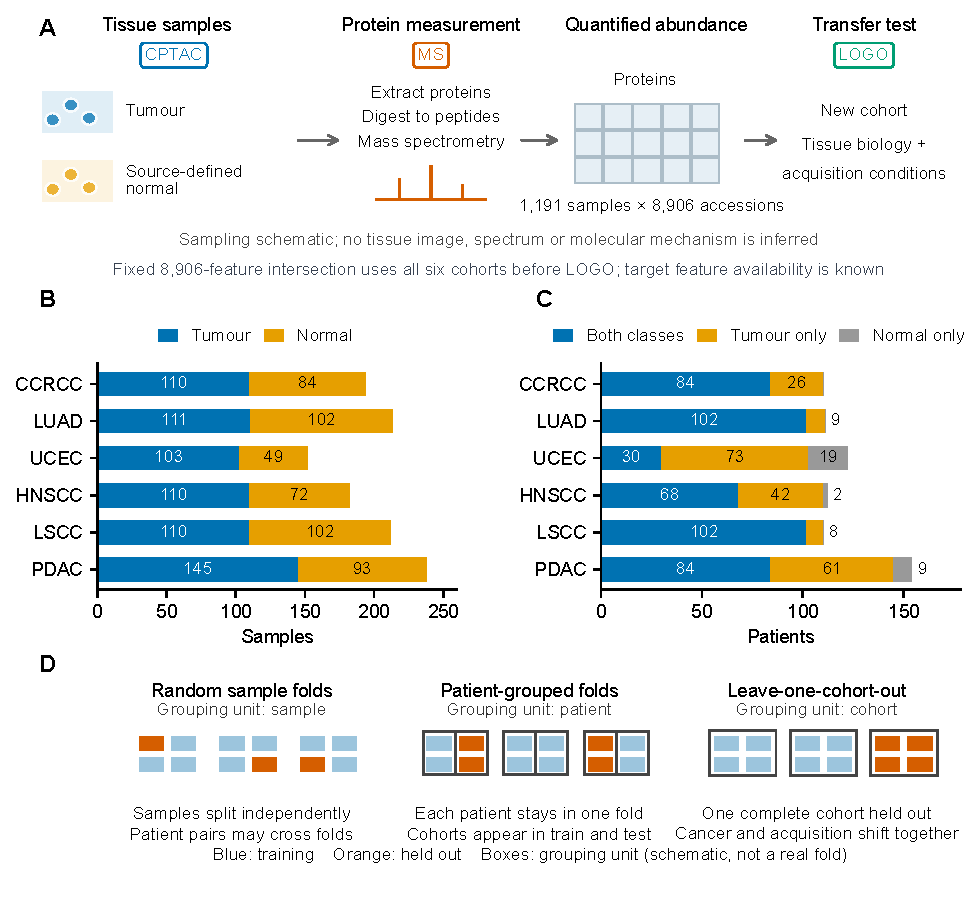
\includegraphics[width=\linewidth]{figures/b28_F0_design.pdf}
\caption{From tissue sampling to cohort transfer. (A) Conceptual path from
tumor and source-defined nonmalignant tissue through mass spectrometry
to the abundance matrix; tissue symbols and peaks are schematic, not
observed histology or spectra. (B) Six cohorts contribute 1,191 samples:
689 tumors and 502 nonmalignant samples, including six HNSCC cored normals.
(C) The 719 true patients include 470 with both tissue classes; some
patients have more than two samples. (D) Sample folds may split a
patient's samples, patient folds keep them together, and LOGO holds out
an entire cancer/study cohort. The blocks illustrate grouping rules,
not actual assignments. The 8,906-feature intersection uses all six
cohorts before LOGO, so target feature availability is known. Cancer
type and study are confounded; the data do not establish one instrument
or one acquisition run per cohort.}
\label{fig:design}
\end{figure}


\section{Results}

\subsection{Accession-aligned abundance improves on descriptive comparators}

The full-abundance LOGO classifier has equal-cohort macro AUROC 0.9343
and separately computed pooled AUROC 0.9555. These are different
estimands: a cohort-average transfer result and a cross-model pooled
ranking statistic. Macro and pooled ECE are 0.1193 and 0.1100,
respectively. The within-cohort AUROCs range from 0.8485 (CCRCC) and
0.8610 (PDAC) through 0.9184 (UCEC) and 0.9809 (HNSCC) to 0.9974
(LSCC) and 0.9998 (LUAD) (Figure~\ref{fig:transfer}).

The missingness comparator has macro/pooled AUROC 0.5445/0.5116, while
the three reference-normalized global summaries reach 0.8172/0.8492.
Thus abundance performs better than either comparator at both levels
of aggregation, but missingness is not exactly uninformative in every
cohort. The high-dimensional model's increment over the three-summary
model is 0.1172 macro or 0.1063 pooled (Figure~\ref{fig:ladder}).
Neither increment is an identified contribution of protein-specific
biology. AUROC differences do not decompose the sources of a signal,
and these summaries are not raw signal-depth measurements.
The first-accession-consistent-gene sensitivity has macro/pooled LOGO
AUROC 0.9329/0.9557, close to the primary accession-aligned analysis
(SI Table~S4).
This is a mapping robustness check on the same samples, not replication.
The identity audit in SI Section S1 is part of the result boundary: the six
HNSCC ``.C'' samples are source-defined cored normals, the corrected manifest
contains 1,191 samples from 719 cohort-scoped patients, and the primary matrix
contains 8,906 stable ENSP accessions. The retired 9,675-name first-protein
mapping selected different stable accessions for 1,234 names; the 8,441-name
analysis is therefore a consistent-accession sensitivity, not an independent
cohort.
Table~\ref{tab:paircounts} gives the corrected tissue composition, and
Figure~\ref{fig:design} links those samples to the three evaluation units.
Neither source-defined normal tissue nor a schematic grouping rule is an
independent clinical validation cohort.

\begin{figure}[tbp]
\centering
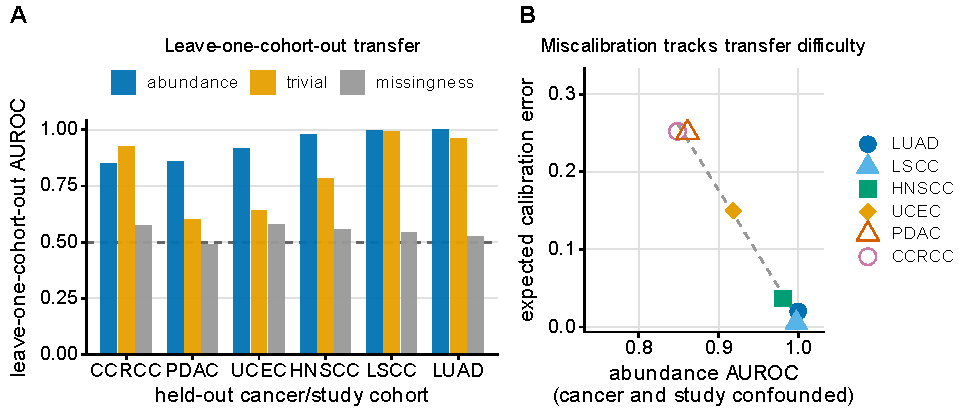
\includegraphics[width=\linewidth]{figures/b28_F1_transfer.pdf}
\caption{Heterogeneous transfer on the corrected six-cohort matrix.
(A) Within-cohort LOGO AUROC for accession-aligned abundance (blue),
three global summaries (orange) and missingness (grey). The dashed line
marks chance ranking. (B) Each cohort's abundance AUROC and ten-bin ECE.
Low-AUROC cohorts have larger calibration errors in this particular
analysis, but no deterministic relation or causal mechanism is inferred.
Each point is a cancer/study cohort; cancer type and study are confounded,
and a cohort is not asserted to be a single acquisition run.}
\label{fig:transfer}
\end{figure}

\begin{figure}[tbp]
\centering
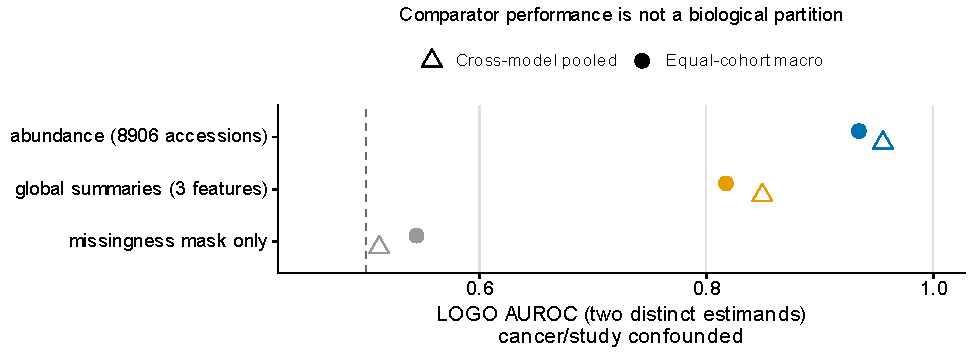
\includegraphics[width=\linewidth]{figures/b28_F2_signal_ladder.pdf}
\caption{Comparator performance is not a biological signal partition.
Filled circles show equal-cohort macro AUROC; open triangles show the
separately computed pooled AUROC, which includes cross-cohort pairs of
scores from different fitted models. Missingness, three global summaries
and 8,906-accession abundance yield macro/pooled values
0.5445/0.5116, 0.8172/0.8492 and 0.9343/0.9555, respectively.
No historical bootstrap whiskers or biological percentages are reused.
Cancer type and study remain confounded.}
\label{fig:ladder}
\end{figure}

\subsection{Calibration error concentrates on harder held-out cohorts}

The three highest-AUROC cohorts have ECE 0.0057 (LSCC), 0.0203 (LUAD)
and 0.0368 (HNSCC). ECE is higher in UCEC (0.1501), PDAC (0.2506)
and CCRCC (0.2522). The reliability curves and probability-error
metrics indicate heterogeneous calibration, not uniform unreliability.
An AUROC--ECE association in six selected cohorts does not show that
poor discrimination forces confident errors. Nor does it distinguish
tissue biology from acquisition differences. Brier scores and log-loss
for the same prediction rows are reported in SI Tables~S1--S3, with their
definitions in SI Section S2. For abundance, CCRCC and PDAC have Brier
scores 0.2245 and 0.2533 and log-loss 0.8162 and 0.7602, compared with
0.0064 and 0.0048, and 0.0253 and 0.0338, for LUAD and LSCC
(SI Table~S1). These complementary errors support the cohort-resolved
description; their relation to ECE is not a mathematical necessity.
All three tables use the same stored predictions, not additional prediction
runs.

\subsection{Random and patient-grouped CV differ from cohort transfer}

Sample CV has macro/pooled AUROC 0.9909/0.9942, and true-patient-grouped
CV has 0.9916/0.9944 (Table~\ref{tab:protocol}). Compared with LOGO, the
sample-CV advantage is 0.0565 macro and 0.0386 pooled. Patient-CV
advantages are 0.0572 macro and 0.0389 pooled. Sample minus patient CV
is $-0.0007$ macro and $-0.0003$ pooled. Preventing patient crossings
therefore does not erase the observed protocol gap in this matrix.
This finding does not isolate a batch effect or establish that patient
structure can never affect performance under another design.

Within fixed cohorts, paired resampling of patients' stored predictions
gives a 0.0442--0.0703 percentile range for the macro sample-minus-LOGO
contrast and 0.0305--0.0478 for its pooled counterpart. These conditional
mixture-sensitivity ranges omit model-refit variability and future-study
uncertainty. They cannot be substituted for a general cross-study CI.
The paired patient draws and their shared protocol contrasts are documented
in SI Table~S7 and Section S5; the ranges are conditional on the corrected patient keys,
not on the historical 723-key partition.

Pooled ECE is 0.0199 for sample CV and 0.0135 for patient CV, compared
with 0.1100 for LOGO. The corresponding macro ECE values are
0.0269, 0.0219 and 0.1193. Figure~\ref{fig:calibration} displays the
reliability curves and pooled calibration errors. The fold scatter in
Figure~\ref{fig:protocol} shows that the difference also concerns
heterogeneity: cohort holdout produces a wider spread of transfer
performance. Those folds have overlapping training sets and are not
independent statistical replicates.

\begin{table}[tbp]
\centering
\caption{Corrected patient and tissue composition. Nonmalignant samples
include both adjacent-normal and HNSCC cored-normal samples. ``Both''
counts patients with at least one sample of each class, not one-to-one
sample pairs. The six HNSCC cored samples are included in its 72 normals.}
\label{tab:paircounts}
\begin{tabular}{lrrrr}
\hline
Cohort & Samples & Tumor/normal & Patients & Both \\
\hline
\tableinput{tables/cohort_rows.tex}
\hline
\end{tabular}
\end{table}

\begin{table}[tbp]
\centering
\caption{Three protocols on the same corrected accession matrix.
Macro is the equal-weight mean of six within-cohort metrics, not the
mean of five CV-fold values. Pooled metrics concatenate all predictions.
Sample CV splits 381 patients across folds; patient CV and LOGO split
none. No protocol here identifies a causal acquisition-batch effect.}
\label{tab:protocol}
\begin{tabular}{lrrrr}
\hline
Protocol & Macro AUROC & Pooled AUROC & Macro ECE & Pooled ECE \\
\hline
\tableinput{tables/protocol_rows.tex}
\hline
\end{tabular}
\end{table}

\begin{figure}[tbp]
\centering
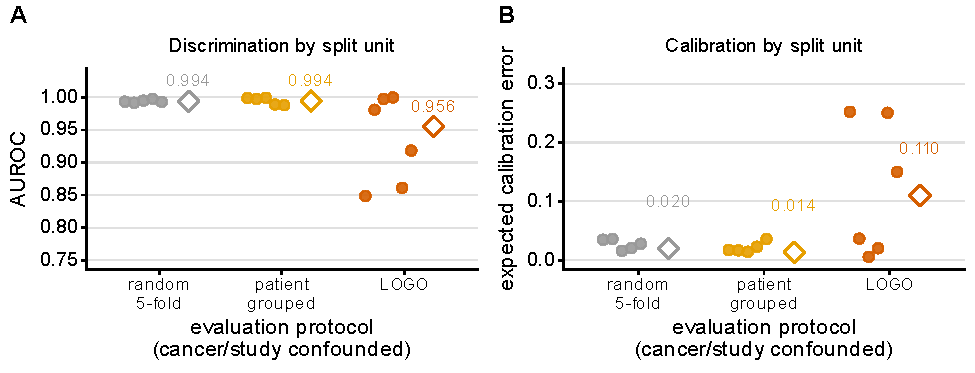
\includegraphics[width=0.92\linewidth]{figures/b28_F5_protocol.pdf}
\caption{Performance depends on the held-out unit. Filled points show
five sample-CV folds, five true-patient folds or six LOGO cohorts;
open diamonds show separately computed pooled metrics. (A) AUROC.
(B) Ten-bin ECE. The pooled values are not averages of the individual
fold values. Fold scatter is descriptive, not a confidence interval;
training sets overlap. Cancer type and study are confounded.}
\label{fig:protocol}
\end{figure}

\subsection{Small pooled sensitivity differences can hide cohort changes}

Full-dataset-median XGBoost has macro/pooled LOGO AUROC 0.9326/0.9543,
compared with 0.9343/0.9555 for training-fold medians. Its pooled ECE
is 0.1144, versus 0.1100. The pooled AUROC change of $-0.00125$ is
small, but CCRCC changes by $+0.00249$ and UCEC by $-0.00693$.
This diagnostic does not justify leaking held-out feature values or
claim that imputation is immaterial in other datasets.

Training-fold-imputed and standardized L2 logistic regression has
macro/pooled AUROC 0.9341/0.9556 and pooled ECE 0.0797. Its pooled
AUROC is only 0.00010 higher than XGBoost, yet CCRCC improves by
0.05520 and PDAC declines by 0.10434 (Figure~\ref{fig:sensitivity}).
Pooled agreement therefore does not imply model-family invariance.
These are matched-cohort sensitivity comparisons, without a claim of
statistical significance for any single cohort's change. SI Tables~S4--S6
retain the cohort-resolved mapping, L2 and deliberately leaky-median
outcomes under the definitions in SI Section S4. All six L2 LOGO fits
converged in 12--44 iterations under the executed 500-iteration limit
(SI Table~S8 and Section S6); convergence does not establish predictive
superiority.

\begin{figure}[tbp]
\centering
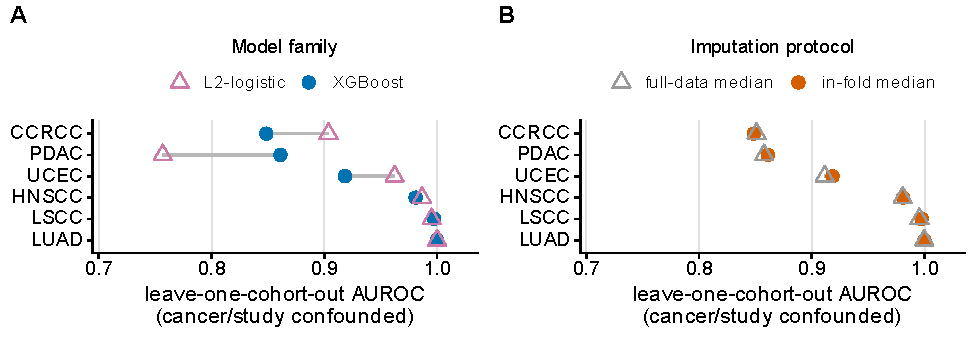
\includegraphics[width=0.92\linewidth]{figures/b28_F6_sensitivity.pdf}
\caption{Cohort-resolved model and imputation sensitivities. (A) XGBoost
versus L2 logistic regression, with training-fold imputation in both and
training-fold standardization for L2. CCRCC AUROC changes from 0.8485
to 0.9037 and PDAC from 0.8610 to 0.7567. (B) Training-fold versus
deliberately full-dataset medians for XGBoost, using identical outer
folds. The same AUROC scale is used in both panels. No interval or
significance claim is assigned to these single-fold comparisons.
Cancer type and study are confounded.}
\label{fig:sensitivity}
\end{figure}

\begin{figure}[tbp]
\centering
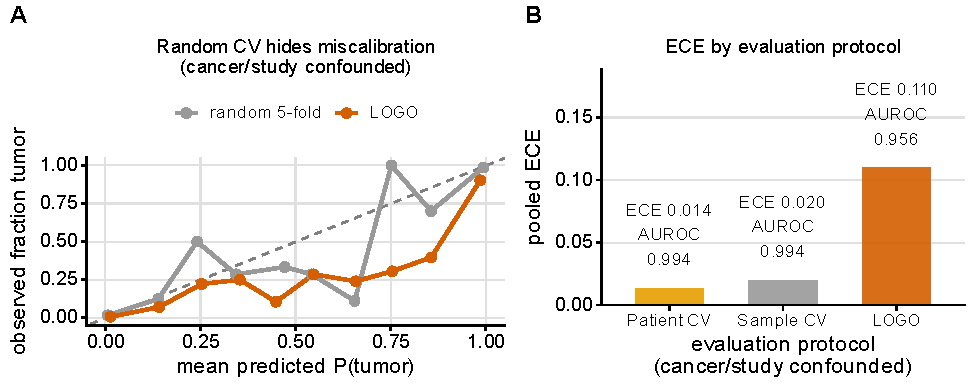
\includegraphics[width=\linewidth]{figures/b28_F3_calibration.pdf}
\caption{Cohort transfer has greater calibration error than cohort-mixing
CV. (A) Mean probability versus observed tumor fraction in ten equal-width
bins; the dashed line denotes perfect calibration. (B) Pooled ECE for
sample CV (0.0199), patient CV (0.0135) and LOGO (0.1100), with pooled
AUROC also shown. ECE uses each bin's sample mass, not equal bin weights.
This is a protocol contrast among confounded cancer/study cohorts.}
\label{fig:calibration}
\end{figure}

\subsection{Confidence-ranked abstention changes cohort composition}

Ranking pooled LOGO predictions by confidence raises retained accuracy
from 0.8497 at full coverage to 119/119 at 10\% requested coverage
(Figure~\ref{fig:abstention}). The top-confidence set contains 52 LUAD,
55 LSCC, six CCRCC, four HNSCC, two PDAC and no UCEC samples.
LUAD and LSCC together comprise 107/119 retained cases. The gain is
therefore accompanied by strong selection of easier cohorts, but the
composition alone does not identify how much improvement comes from
between-cohort selection versus within-cohort case ranking. In particular,
PDAC is not entirely absent from the retained set, contrary to the
historical result. The complete composition is given in
Table~\ref{tab:cohortcomp}.

Selective classification \citep{GeifmanSelective} and calibration answer
different questions. This retrospective curve does not repair
probability calibration, validate a deployment threshold, or ensure
reliability on a new PDAC- or UCEC-like population. Neither 119/119
correct retained predictions nor their pooled composition supplies a
clinical performance guarantee.

\begin{table}[tbp]
\centering
\caption{Cohort fractions in the confidence-ranked retained set.
Rows use the same stored LOGO predictions as the accuracy curve.
Requested coverage is rounded down to an integer retained count.}
\label{tab:cohortcomp}
\small
\begin{tabular}{lrrrrrrr}
\hline
Coverage & $n$ & CCRCC & LUAD & UCEC & HNSCC & LSCC & PDAC \\
\hline
\tableinput{tables/coverage_rows.tex}
\hline
\end{tabular}
\end{table}

\begin{figure}[tbp]
\centering
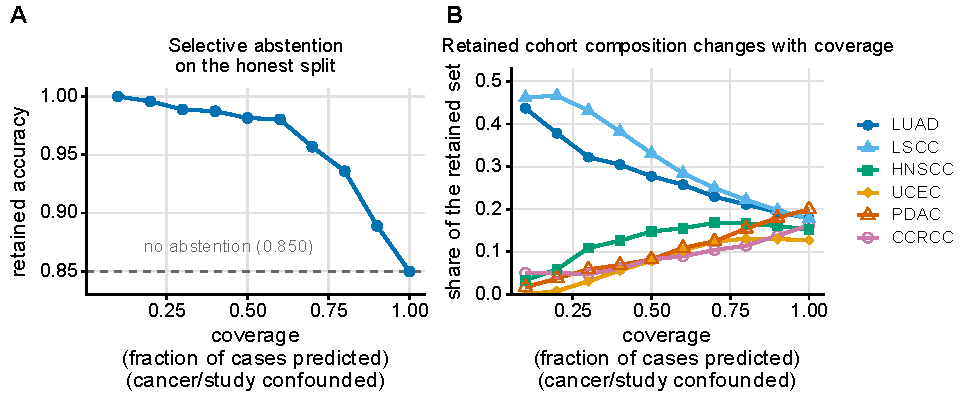
\includegraphics[width=\linewidth]{figures/b28_F4_riskcoverage.pdf}
\caption{Retained accuracy and retained populations change together.
(A) Accuracy among the highest-confidence LOGO predictions; the dashed
line is full-coverage accuracy 0.8497. (B) Cohort fractions in the same
sets. At 10\% coverage, LUAD and LSCC account for 52/119 and 55/119
samples; PDAC contributes 2/119 and UCEC contributes none. The curves
do not isolate within-cohort triage effects or validate an operational
abstention rule. Cancer type and study are confounded.}
\label{fig:abstention}
\end{figure}

\subsection{A specific recalibration procedure has cohort-dependent effects}

On the corrected outer LOGO predictions, split-half temperature scaling
reduces pooled ECE from 0.1100 to 0.0845 and Platt scaling to 0.0388.
Corresponding pooled Brier scores are 0.1135 before calibration, 0.0998
after temperature scaling and 0.0839 after Platt scaling. The cohort
breakdown in Table~\ref{tab:recal} shows uneven effects: for example,
Platt ECE falls from 0.2522 to 0.1303 on CCRCC but rises from 0.0203
to 0.0272 on LUAD.

The fitted temperatures range from 1.5506 to 2.0296 and all soften
the probabilities (Figure~\ref{fig:temperature}). This describes these
six fitted maps, not an intrinsic restriction of temperature scaling,
which can also sharpen probabilities when $T<1$. The calibration fit
uses inner two-/three-cohort predictors rather than the outer
five-cohort training regime. Consequently, heterogeneous benefit is a
result for this procedure, not proof that a single recalibration method
must fail under every transfer design. No held-out label was used to
fit the maps. The inner split construction and bounded temperature/Platt
fits are specified in SI Section S6, so this is a defined recalibration
procedure rather than an unspecified post-hoc correction.

\begin{figure}[tbp]
\centering
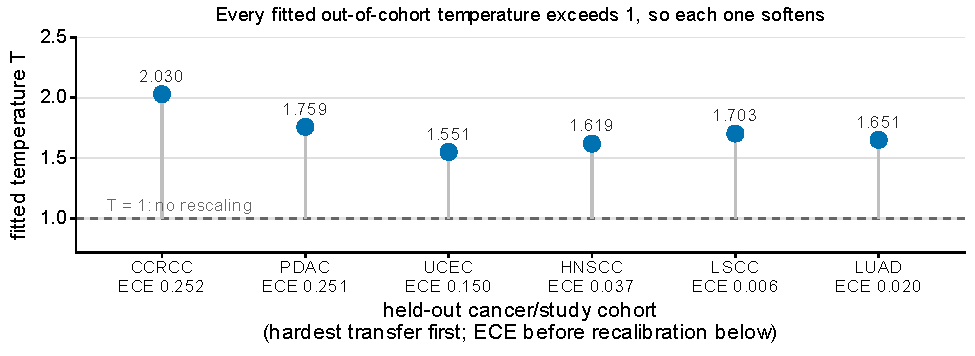
\includegraphics[width=\linewidth]{figures/b28_F7_temperature.pdf}
\caption{Temperatures fitted without outer held-out labels. All six
estimated temperatures exceed one in this analysis; the dashed line
denotes no rescaling. The printed ECE values are before recalibration.
The calibration predictors trained on two or three cohorts, while the
outer predictor trained on five. These maps therefore evaluate one
specified inner/outer procedure. Per-cohort outcomes and the Platt
alternative are in Table~\ref{tab:recal}. Cancer type and study are
confounded.}
\label{fig:temperature}
\end{figure}

\begin{table}[tbp]
\centering
\caption{Ten-bin ECE for the same outer LOGO predictions before and after
the specified split-half recalibration procedure. Each cohort has its
own map fitted using other cohorts only; pooled ECE is recomputed after
concatenation, not averaged over these rows.}
\label{tab:recal}
\begin{tabular}{lrrr}
\hline
Cohort & Before & Temperature & Platt \\
\hline
\tableinput{tables/recalibration_rows.tex}
\hline
\end{tabular}
\end{table}

\subsection{What the protocol contrast does not identify}

The study does not identify a biological or technical fraction of the
observed transfer performance. Each primary group corresponds to a
distinct cancer/study cohort; the source metadata do not establish that
each is a single acquisition batch. An observed sample/patient-versus-cohort
contrast can motivate choosing a relevant evaluation unit without
identifying why an individual cohort is hard.

The separately recorded OV side-study is retained as historical context:
its archived summary reports pooled plex-LOGO abundance AUROC 0.985, close to random five-fold
AUROC 0.987, with plex-LOGO ECE 0.046 and global-summary AUROC 0.951.
It has only 103 samples, including 19 normals distributed as one to
three per plex. It is one cancer type, a different feature table and a
different holdout unit. The reported near-zero protocol contrast is not a
prediction-replayed counterexample or a deconfounding test of the six-cohort result.
The current fixed six-cohort comparison does not establish a universal gap;
that restriction does not depend on treating the OV summary as verified new evidence.
These are retained historical summary values with checked source
provenance, not newly replayed OV predictions.

Numerical claims from historical six-cohort identification diagnostics,
synthetic shifts, representation transforms and the separate dual-platform
mapping are not used to strengthen the corrected primary conclusion.
Their assumptions and current evidence status are itemized in SI Section
S7, with the reproducibility boundary in Section S8. In particular, a
label-dependent residual
construction would not be a deployment evaluation, and a two-way
variance calculation on a confounded design would not by itself
identify biological and acquisition contributions. No pathway-enrichment
analysis was performed.


\section{Discussion}

The central interpretation is about evaluation units. A random split
can be internally consistent and still answer a less demanding question
than transfer to a new cancer/study cohort. In this corrected six-cohort
matrix, both random and true-patient-grouped CV yield higher
discrimination and lower calibration error than cohort holdout.
The common accession panel was defined with knowledge of which features
occur in the held-out cohort. This is not label leakage, but the
contrast conditions on target-cohort feature availability; an unseen
cohort with a prospectively locked panel remains unevaluated here.
Patient grouping closes the identified patient-identity defect without
erasing the contrast. It does not separate cancer-type biology from
study-specific acquisition conditions.

The distinction between macro and pooled performance is consequential.
Pooled AUROC combines scores from different fitted models and
cross-cohort positive--negative pairs; the macro result averages
within-cohort ranking. Neither should be silently substituted for the
other. Fixed-prediction patient resampling gives a useful sensitivity
to the sampled patients within these six studies, but not a complete
uncertainty analysis of refitted learning procedures or future cohorts.

Global abundance summaries and missingness controls constrain
interpretation of the high-dimensional model without converting AUROC
increments into biological shares. Correct accession identity is
necessary for this comparison; choosing the first protein associated
with each gene does not guarantee a shared protein feature across
cohorts. The source-normalized measurement scale also prevents the
three-summary model from being described as a raw total-signal assay.

The imputation and model-family sensitivities show why similar pooled
performance is insufficient evidence of invariance. L2 and XGBoost
have almost the same pooled AUROC, but differ substantially on CCRCC
and PDAC. Calibration and selective prediction likewise require
cohort-resolved reporting: improved retained accuracy is accompanied
by a changed cohort mixture, and the specified recalibration maps help
some cohorts more than others. Neither supplies a deployment guarantee.

The correction and evaluation questions should remain separate.
BERNN uses unlabeled validation and test features during representation
warm-up \citep{PelletierBERNN}; its reported protocol is not an
interchangeable numerical baseline for the transfer fits here. We have
not benchmarked BERNN or pipeML \citep{HurtadoPipeML} head-to-head and
make no superiority claim. A future harmonization comparison should
state whether unlabeled target features are available and report
calibration as well as discrimination. Our rejection curves are not
conformal prediction sets and have no finite-sample coverage guarantee
under cohort shift.

Tumor-versus-normal is a high-effect testbed, not a clinically actionable
biomarker task. Six selected cohorts from one CPTAC processing source
do not establish multi-platform generality. The separate OV summary is
historical context without prediction-level replay in this revision;
it is not independent evidence for or against the six-cohort contrast.
Historical diagnostics on the superseded feature matrix remain
archived but cannot substitute for new evidence after identities change.
Independent measurements crossing cancer type with acquisition
environment, broader model comparisons, and full refit-based uncertainty
would be needed for stronger transfer claims.

The practical recommendation is to align the evaluation unit with the
intended use, report within-cohort discrimination, calibration and
coverage together, and distinguish macro from pooled summaries.
The corrected data still support a protocol contrast in this design.
They do not establish a general biological transfer law or identify a
causal batch effect.

\section{Supporting Information}
The accompanying Supporting Information gives corrected sample and
feature definitions, cohort-resolved AUROC and probability errors,
conditional resampling ranges, L2 convergence checks, and an explicit
disposition of historical side studies. Its tables and the main-text
tables are generated from the same verified prediction records.

\section{Data Availability Statement}
All biological inputs are public CPTAC tables accessed through
\texttt{cptac} \citep{cptacPkg}. The primary analysis uses the
\texttt{umich} source for CCRCC, LUAD, UCEC, HNSCC, LSCC and PDAC.
No new biological data were generated.

The current code and research artifacts are available at
\url{https://github.com/PeterPonyu/b28-proteomics-transfer}, release tag
\texttt{author-review-2026-10-02}, with the version-specific archive
\url{https://doi.org/10.5281/zenodo.23101188}. The package contains this
Article and Supporting Information, their source and figure inputs,
corrected sample/patient/fold and accession maps, stored predictions,
analysis and verification programs, software environment records and a
SHA-256 inventory. Dated candidate filenames retain their provenance;
the current public manifest binds the included files to this revision.
Default offline checks verify stored predictions and metrics and render
the supplied PDFs without fitting models or downloading assay data.

A complete scientific rerun requires separately acquired, matching
CPTAC/UMICH abundance and mapping files and the recorded fit environment.
\texttt{DATA\_SOURCES.md} records cohort/source/loader versions, filenames
and input hashes; unrecorded PDC study accessions and per-cohort version
labels are explicitly identified as unknown. Third-party raw proteomics
are not redistributed. Author-owned code is MIT licensed; authored text,
figures and derived result tables are CC BY 4.0 to the extent of author
rights. Upstream conditions remain applicable as detailed in
\texttt{THIRD\_PARTY\_NOTICES.md}. The earlier archive
\url{https://doi.org/10.5281/zenodo.21870024} is historical, not the
current corrected release. Artifact publication does not constitute
independent scientific or clinical validation.


\section*{Author Information}

\noindent\textit{Corresponding Author.}
Zeyu Fu --- State Key Laboratory of Trauma and Chemical Poisoning, Institute of Combined Injury, Chongqing
Engineering Research Center for Nanomedicine, College of Preventive Medicine, Army Medical University, Chongqing,
China; ORCID 0009-0001-8329-0108; email \href{mailto:fuzeyu99@126.com}{fuzeyu99@126.com}.

\noindent\textit{Notes.}
The author declares no competing financial interest. Funding: N/A --- no external funding to declare.
Acknowledgments: N/A.

\bibliography{ref}

\end{document}
